\chapter{Experiment Construction}
\label{chapter:construction}
This chapter describes the implementation of the applications studied in the experiments. The workload application was inspired by the Canny edge detector. Two versions of the workload were implemented and both were instrumented for measurement. Three experiments were designed for comparison of the applications.

To begin this chapter the general idea of the workload application is introduced in~\ref{sec:filterapp}. Then the PREESM implementation of the application is described in~\ref{sec:preesmapp}. Next the OpenEM implementation is explained in~\ref{sec:oemapp}. After the applications have been described, the instrumentation explained in~\ref{sec:instrumentation}. Finally the experiments introduced in~\ref{sec:experiment-description}.

\section{Filter Application}
\label{sec:filterapp}
The objective of this thesis is to study the suitability of OpenEM framework for building stream processing applications. Video streams make up an increasing proportion of the data being transferred in the Internet. The processing of video streams requires a lot of computing power, as the streams have increasingly high bit rates and they have to be compressed for transfer and storage. The high performance requirements of processing video streams make them interesting for research and for this reason they were selected as the stream format used in this thesis.

Three requirements for the workload applications were specified to guide the design. The requirements are presented in the following list.

\begin{enumerate}
    \item{Variable input bit rates}
    \item{Comparability the PREESM and OpenEM applications}
    \item{Highly analyzable}
\end{enumerate}

\textbf{Variable input bit rates} were required of the workload applications to make it possible to study the performance of the OpenEM framework in processing dynamic workloads. Varying the bit rates of the video stream inputs is simple as the frame size of the stream is easy to change and it doesn't affect the algorithms used in any unforeseeable way. \textbf{Comparability of the PREESM and OpenEM applications} was required so the PREESM workload could be used as a baseline implementation. Last requirement for the applications was that they needed to be \textbf{highly analyzable} in order to enable the study of OpenEM performance. An application satisfying these requirements was designed using the PREESM Sobel example at \cite{preesmtut} as the starting point and adding another processing component to it.

It is important to notice that the actual performance of the filter application in its nominal video filtering task was mostly disregarded. For example the data is copied to a new buffer in every processing stage and the filter algorithms are not optimized for the specific platform. Therefore, comparing the performance of the implemented applications to real world implementations of similar applications is not useful.

The idea for using Sobel and Gauss filters in the same application came from the Canny edge detector. However, the filters in the workload applications are executing independently of each other on separate video streams, unlike how they are connected in the Canny edge detector.

\section{PREESM Filter Application}
\label{sec:preesmapp}
An actor network that represents the video filter application is constructed in PREESM. The final PiSDF model of the PREESM video filter application is presented in figure \ref{fig:preesm_actors}. The PREESM filter application is adapted from the PREESM example in \cite{preesmtut} by adding another processing path for the Gaussian filter and making the necessary modifications to the shared parts of the application.

\begin{figure}[h!]
    \begin{center}
        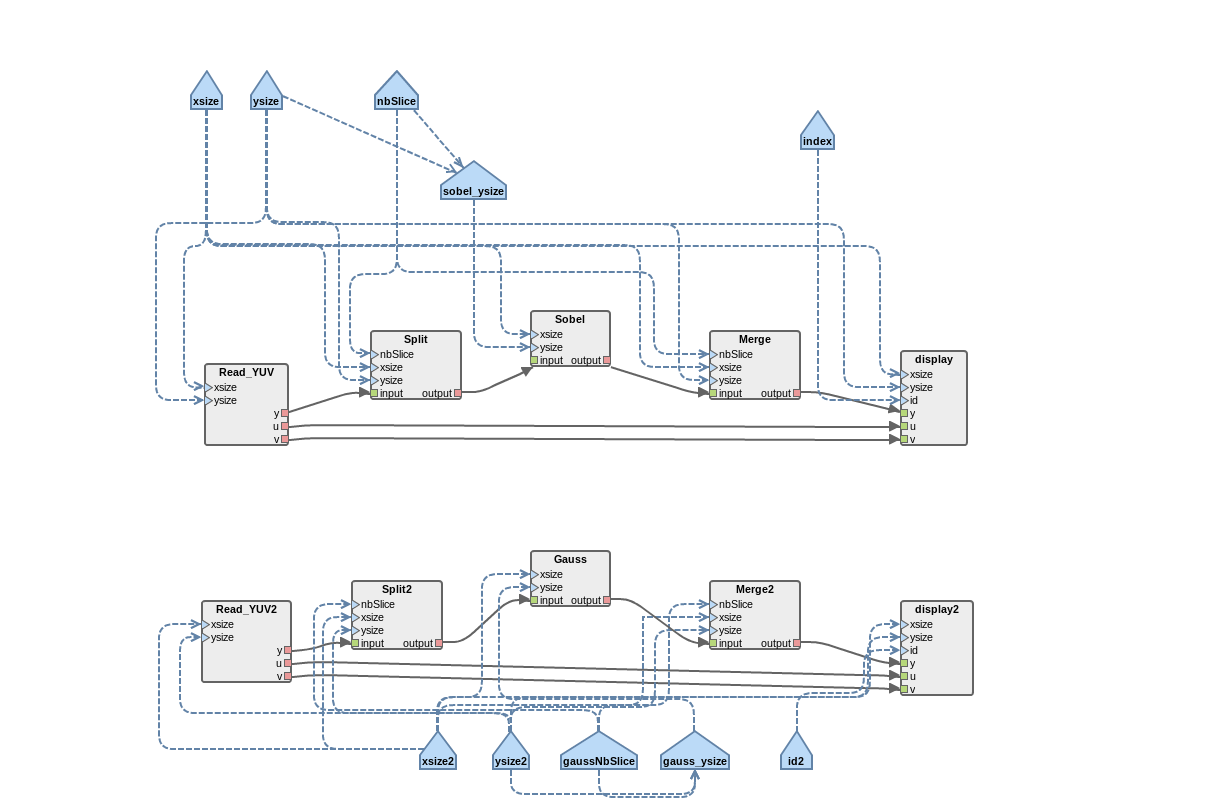
\includegraphics[width=0.99\textwidth]{images/preesm_diagram.png}
        \caption{The PiSDF graph of the PREESM filter application}
        \label{fig:preesm_actors}
    \end{center}
\end{figure}

\subsection{Actor Model}
\label{subsec:actors}
To keep the model simple and the program well analyzable both of the processing paths in the network are independent. The first actor on both of the processing paths, the \textit{Read\_YUV} and the \textit{Read\_YUV2} actors in the figure \ref{fig:preesm_actors}, loads the video frames from memory and passes them to splitting actors. The \textit{Split} actors split the frames to a suitable number of slices to enable processing of the same video stream on multiple cores. The filter actors, \textit{Sobel} and \textit{Gauss} in the figure, follow the \textit{Split} actors. Partial frames filtered in the filter actor are merged back into whole frames in the \textit{Merge} actors. The last actors on both of the processing paths, called \textit{display} and \textit{display2}, are dummy actors.

The pentagons in the top and the bottom of the figure represent the parameters of the application. The \texttt{xsize}, \texttt{ysize}, \texttt{xsize2} and \texttt{ysize2} parameters specify the size of the input frames. \texttt{nbSlice} and \texttt{gaussNbSlice} determine the numbers of slices the frames are split to. The \texttt{sobel\_ysize} and \texttt{gauss\_ysize} are the heights of the slices after splitting.

The first actors \textit{Read\_YUV} and \textit{Read\_YUV2} call the \texttt{readYUV} function defined in the PREESM example at \cite{preesmtut}. IO is omitted from the application, as it is not in the scope of the experiments. The processing starts with loading the frames from memory. In a real world application the frames would be written to the memory for example with DMA by a packet processor processing a stream of network packets. The \texttt{readYUV} function copies the Y component of the input frame to the output address while the U and V components are ignored. The U and V are omitted because the \textit{Sobel} and \textit{Gauss} actors only operate on the Y channel in the experiment setup.

The \textit{Split} actor operates on the output of the \textit{Read\_YUV} actor. The \textit{Split} actor preprocesses the frame for the \textit{Sobel} and \textit{Gaussi} actors. Since the Sobel and Gauss filters involve convolution with 3x3 and 5x5 matrices respectively, they will need to access image data outside the part of the image they are processing. To enable parallel processing of a single frame on multiple cores, the frame is split in to slices. These slices will also need to contain a bit of extra data so that the filters can operate correctly. Black lines, meaning lines with the Y value of 0, are added to the top and the bottom of the frame. One black line is enough for the Sobel frames but two black lines are needed for the Gaussian frames, corresponding to the filter kernel sizes. After the padding, the slices overlap each other for one or two lines again corresponding to the size of the filter kernel. With the black lines added the frame is copied to the output buffer one slice at a time.

The \textit{Sobel} actor calculates the convolution of the Sobel kernels presented in \ref{fig:sobelmat} on the Y component of the input frame. The \textit{Sobel} actor from the PREESM example at \cite{preesmtut} is used in this experiment. The convolution is computed by looping over the pixels in the input frame, calculating the $G_{x}$ and $G_{y}$ components of the Sobel operator and combining them by computing the average of absolute values of $G_{x}$ and $G_{y}$. After looping over the image the actor overwrites the edges of the frame with black pixels.

The \textit{Gauss} actor operates similarly to the \textit{Sobel} actor but instead of closed expressions, the value of the filter function at each points is calculated by looping over the neighboring pixels and multiplying the intensity values by the corresponding weight from the Gaussian kernel presented in \ref{fig:gaussmat}.

The last actor processing the frame is the \textit{Merge} actor. The \textit{Merge} actor copies the processed data from its input buffer to its output buffer, overlaying the slices so that the output frame does not contain the extra lines created in the \textit{Split} actor. Since there is no real IO in the application, the merged frame is not processed further. In a real world application the processed frame would be copied for example to a network packet. As there is no IO the \textit{Display} actors do not do any computations. In the experiments the \textit{Display} actor is used as the endpoint of the processing and it starts the data export.

\subsection{PREESM Schedule}
\label{subsec:preesmsched}
The scheduler of the PREESM framework is described in \ref{sec:preesm-scheduling}. The scheduler creates a block schedule from the actor model using user provided estimates for the actor durations. To get reasonably accurate estimates, the application was first scheduled with the default values and the actor durations were measured on the target device. The resulting timings are presented in the table \ref{tab:preesm_times}. The timings from the measurements were approximately the same for all the actors except for the \textit{Gauss} actor. A Gantt chart representing the schedule, created using the values in the table, is presented in figure \ref{fig:preesm_gantt}. The mutable parameters in the application, presented in the graph \ref{fig:preesm_actors}, affect the static memory allocations of the PREESM application. This makes it necessary to execute the PREESM codegen workflow every time the parameters are changed. For this reason, the PREESM schedules of the different measurement setups are slightly different.

\begin{table}
    \begin{center}
        \begin{tabular}{| c | c |}

            \hline
            Cycles & Actor \\ \hline
            600 & Gauss \\ \hline
            150 & Merge \\ \hline
            150 & Merge2 \\ \hline
            150 & Read\_YUV \\ \hline
            150 & Read\_YUV2 \\ \hline
            150 & Sobel \\ \hline
            150 & Split \\ \hline
            150 & Split2 \\ \hline
            1 & display \\ \hline
            1 & display2 \\ \hline
        \end{tabular}
        \caption{PREESM Actor Timings.}
        \label{tab:preesm_times}
    \end{center}
\end{table}

The PREESM framework does not support changing the timing of the implode and explode operations, which was found in the experiments to start affecting the schedule considerably with larger frame sizes. The duration estimates used by PREESM for the implode and explode operations are very short compared to durations of the actors measured from the application. The explode operations for both streams are represented in the Gantt chart by the small time slices preceding \textit{Gauss} actors on cores 4 and 7. The implode operation for Gauss stream follows the \textit{Gauss} actor execution on core 7 and the implode operation of Sobel stream follows the latter \textit{Sobel} actor on core 5.

\begin{figure}[h!]
    \begin{center}
        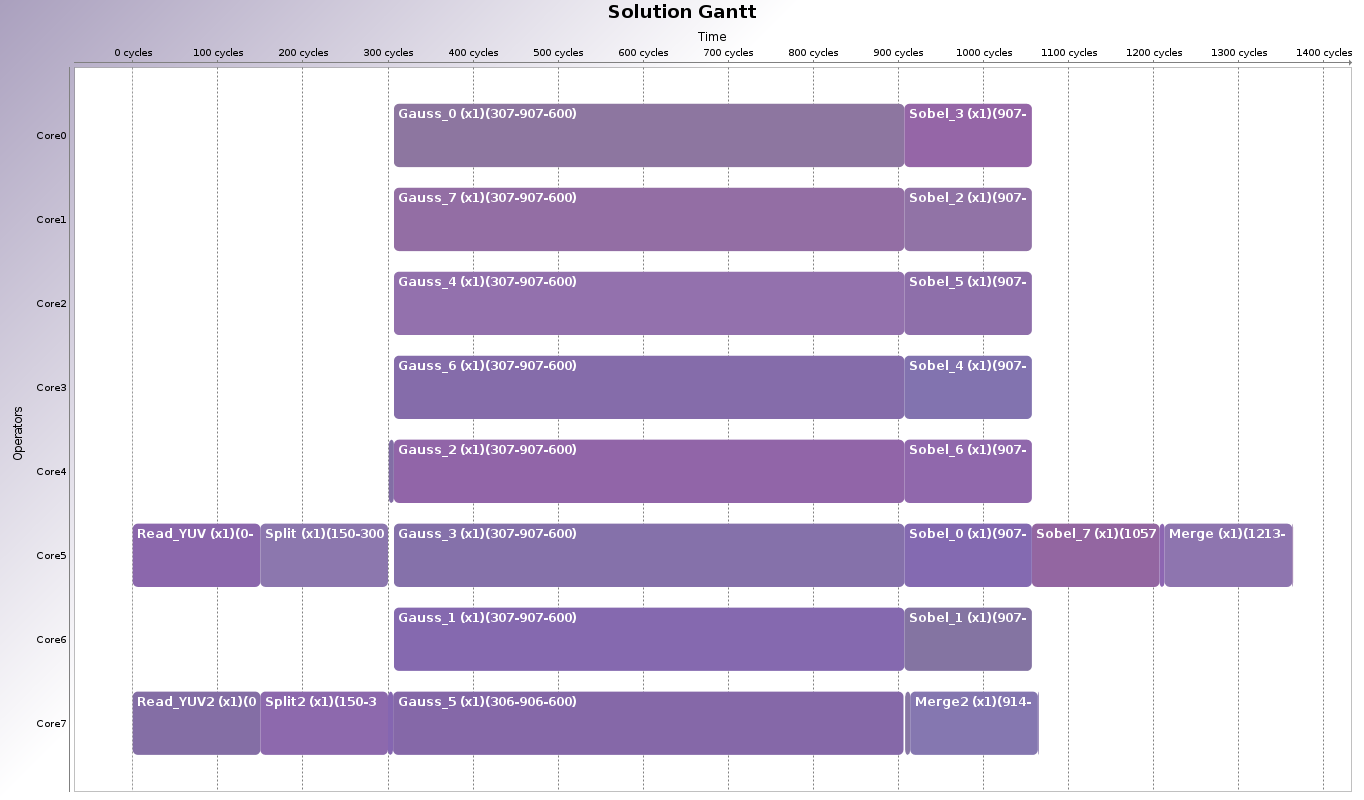
\includegraphics[width=0.99\textwidth]{images/gantt_preesm_cifcif.png}
        \caption{Gantt chart representing the schedule of a PREESM Filter Application.}
        \label{fig:preesm_gantt}
    \end{center}
\end{figure}

A block schedule could be generated, which would yield a higher throughput by introducing multiple instances of the actors for each repetition of the schedule. The successive repetitions of the schedule would be interleaved and the overhead of synchronizing the cores would be reduced. The current version of PREESM does not support the described interleaving of the repetitions \cite{pelcat2014preesm}.

\section{OpenEM Filter Application}
\label{sec:oemapp}
The OpenEM implementation of the filter application was designed using the PREESM filter application as the starting point. Specifically, the OpenEM application has to process the frames in a similar manner, so that ideally only the scheduling policies between the two programming models would differ. The high-level structure of the OpenEM filter application is presented in the figure \ref{fig:openem_flow}. The application consists of two atomic queues, a parallel queue, and three execution objects. Each queue is connected to only one execution object. The execution runs in cycles. A new cycle is started every time the previous cycle finishes. There are multiple cycles running in parallel, but since the read and merge EOs are atomic, only filter EO is running on multiple cores in parallel.

The design principles introduced in the beginning of this chapter apply to the OpenEM application as well. The OpenEM application was not designed for maximum performance but to demonstrate the suitability of OpenEM as a platform for stream processing applications. The performance of the application could be improved in many ways, for example, by minimizing the amount of redundant copying of the frame slices and introducing parallelism to frame reading and merging.

\begin{figure}[h!]
    \begin{center}
        \usetikzlibrary{chains}

\begin{tikzpicture}[>=latex,node distance=0pt, scale=0.7, every node/.style={transform shape}]
    % the rectangular shape with vertical lines
    \node[rectangle split, rectangle split parts=6,
    draw, rectangle split horizontal,text height=0.5cm,text depth=0.5cm,inner sep=0pt, text width=0.0cm] (atomic1) {};
    \fill[white] ([xshift=-\pgflinewidth,yshift=-\pgflinewidth]atomic1.north west) rectangle ([xshift=-5pt,yshift=\pgflinewidth]atomic1.south);

    \node[draw,ellipse,right= 0pt of atomic1,minimum height=1.0cm,inner xsep=5pt] (readEO) {Read EO};

    \node at (5, 0)[rectangle split, rectangle split parts=6,
    draw, rectangle split horizontal,text height=0.5cm,text depth=0.5cm,inner sep=0pt, text width=0.0cm ] (parallel) {};
    \fill[white] ([xshift=-\pgflinewidth,yshift=-\pgflinewidth]parallel.north west) rectangle ([xshift=-5pt,yshift=\pgflinewidth]parallel.south);

    \node[draw,ellipse,right= 0pt of parallel,minimum height=1.0cm,inner xsep=5pt] (filterEO) {Filter EO};

    \node at (10, 0)[rectangle split, rectangle split parts=6,
    draw, rectangle split horizontal,text height=0.5cm,text depth=0.5cm,inner sep=0pt, text width=0.0cm] (atomic2) {};
    \fill[white] ([xshift=-\pgflinewidth,yshift=-\pgflinewidth]atomic2.north west) rectangle ([xshift=-5pt,yshift=\pgflinewidth]atomic2.south);

    \node[draw,ellipse,right= 0pt of atomic2,minimum height=1.0cm,inner xsep=5pt] (mergeEO) {Merge EO};

    % the arrows and labels
    \draw [->](readEO) to (parallel);
    \draw [->](filterEO) to (atomic2);
    \draw [->](mergeEO) .. controls (16,0) and (15, 2) .. (6, 2) .. controls (-2, 2) and (-3, 0) .. (atomic1);

    \node[align=center,below] at (atomic1.south) {Atomic Queue};
    \node[align=center,below] at (parallel.south) {Parallel Queue};
    \node[align=center,below] at (atomic2.south) {Atomic Queue};
\end{tikzpicture}

        \caption{The OpenEM filter application.}
        \label{fig:openem_flow}
    \end{center}
\end{figure}

The application execution starts with initializing the OpenEM framework and the application data structures. The OpenEM initialization is explained in \ref{subsec:ti-init-layer}. After the queues and the execution objects have been initialized the application creates a number of initial events that are sent to the read queue. Once the events have been queued the application synchronizes all cores and the actual execution starts.

The Read EO combines the functionality of the \textit{Read} and \textit{Split} actors of the PREESM filter application presented in \ref{fig:preesm_actors}. A frame is read from the input video memory and split into a number of slices. The functions called are exactly the same as in the PREESM application. The frame slices are copied to event buffers of new events. The new events are then sent to the filter queue. There is only one filter queue and one filter execution object. The same execution object will compute either Sobel or Gauss filter on the frame slice according to its type.

The PREESM application splits the frames into slices and processes the slices separately before merging them back into one frame. Similar fork-join mechanism was implemented in the OpenEM application. Frames are accumulated simply in a merge buffer located in shared memory, which is referenced through queue context pointers. The bookkeeping for frame completion is handled in the shared memory as well.

The filtered frame slices are accumulated in the merge buffer, which is accessed through the merge queue context. The merge queue is atomic to avoid need for synchronization between the cores. After a frame has been merged the merge EO creates a new event, which is sent to the read queue. The ratio of Sobel filtered frames to Gauss filtered frames is always one to one.

\section{Instrumentation}
\label{sec:instrumentation}
To understand the behavior and performance of the applications their execution needs to be measured. The measurements conducted in the experiments are based on cycle counts. The TMS320C6678 exposes cycle counts on each core through two registers, namely TSCL and TSCH, which store the low 32 bits and the high 32 bits of the cycle count respectively. Comparing the values of the TSCL register in the beginning and the end of processing on each core gives accurate local timings and would be enough for measuring the execution on single core. However, for accurate measurements of global cycles, the cycle offsets to the global cycle count need to be stored. The functionality for counting cycles is included in the Texas Instruments OpenEM initialization and utilities code. The cycle counts are stored in the DDR memory.

The latency of both of the filters is measured from the time the frame is loaded from the memory to the time the frame is merged after filtering. The throughput is measured as frames per second processed in total by the application. Since both of the applications process frames at the same rate from both streams, there is only one FPS measurement for each of the measurement setups.

In the PREESM application the cycle counts are saved in the beginning and the end of each user defined function of the application. In addition to this total cycle count was measured in the \texttt{readYUV} function. In the OpenEM application cycle counts are measured over the same functions as in the PREESM application and in the beginning and in the end of each EO. The latter measurements are carried out to get a better understanding of the OpenEM runtime overhead.

The measurements are exported through the debug connection of the TMS320C6678 using IO library provided by Texas Instruments.

\section{Description of Experiments}
\label{sec:experiment-description}
In these experiments, the OpenEM and PREESM filter applications are loaded with similar workloads and their execution is measured. The idea of the experiments is to examine the dynamic scheduling capabilities of the OpenEM scheduler and the overhead of the OpenEM framework in stream processing. The OpenEM scheduler is hardware accelerated, running on a separate processor in the TMS320C6678 chip. The scheduling is explained in detail in chapter \ref{chapter:openem}. To achieve this objective the OpenEM filter application introduced in chapter \ref{chapter:construction} is measured under different loads and compared to a similar application implemented using PREESM. The PREESM application should be considered a baseline, which demonstrates how a statically scheduled application behaves under dynamic workload.

The static schedule of the PREESM application is regenerated between every measurement setup due to the limitations of the code generation in PREESM framework. The specific limitation is that the parameters of the actor model are translated into static memory allocations in the code generator, and manually changing the generated allocations would be complicated and prone to error. As a result the actors are scheduled slightly differently between each scenario. The schedules differ in the mapping of actors to cores but not in the ordering of the actors. The actor ordering is defined by the dependencies between the actors and availability of computing resources. The estimated actor timings of the PREESM application are not modified when changing the frame size.

In the experiments the applications are loaded with three different workloads and measured. In addition the OpenEM application is measured under the same load but different numbers of available cores. The experiments are described in the following subsections. In the first subsection the parameters and factors of the experiment are introduced. Second the different measurement setups are described and third the results of the experiment are presented.

\subsection{Parameters and Factors}
\label{subsec:parameters-and-factors}
Dynamic workload conditions are emulated by repeating the measurements with different factors. To keep the measurement setup simple the video streams are not dynamically switched at runtime. The measurement parameters are presented in the following listing.

\begin{itemize}
    \item \textbf{Video Frame Size} - Changing the frame sizes of the video streams differentiates the workloads.
    \item \textbf{OpenEM Core Masks} - The OpenEM application is measured with different core masks of the Execution Objects.
    \item \textbf{Number of Frames Processed Simultaneously} - The OpenEM application processes variable number of frames simultaneously.
\end{itemize}

The different video frame sizes used are presented in table \ref{tab:cif_frames}. The frame sizes used are selected from among the Common Intermediate Format frame sizes. YUV video format is used in the applications, but only the Y channel is processed by the applications. The Y channel in the YUV frame contains $R_{x} * R_{y}$ bytes where $R$ is the resolution. In the YUV format used the U and V channels have reduced bit rates of $\frac{1}{4} * R_{x} * R_{y}$ per frame.

\begin{table}
    \begin{center}
        \begin{tabular}{ c c c }
            Name  & X resolution  & Y resolution \\ \hline
            QCIF  & 176           & 144          \\ \hline
            CIF   & 352           & 288          \\ \hline
            4CIF  & 704           & 576          \\ \hline
        \end{tabular}
        \caption{CIF frame sizes}
        \label{tab:cif_frames}
    \end{center}
\end{table}

The OpenEM application circulates the events created initially throughout its lifetime. The number of initial events determines the maximum number of frames that can be processed simultaneously. The effect of the number of the simultaneously processed frames to the latency and throughput of the application is examined in the experiments.

OpenEM core masks are used to limit the number of cores available to the filter application. The behavior of OpenEM is examined under limited resources. With the use of core masks the performance improvement through increased parallelism is investigated.

\subsection{Measurement Setups}
\label{subsec:measurement-setups}
The filter applications process two video streams simultaneously as described in chapter \ref{chapter:construction}. One video stream is processed with a Sobel filter and the other is processed with a Gaussian filter. The dynamic behavior of the applications is investigated using different workloads.

\begin{table}
    \begin{center}
        \begin{tabular}{ c c }
            Sobel Resolution & Gauss Resolution \\ \hline
            CIF              & CIF              \\ \hline
            4CIF             & CIF              \\ \hline
            CIF              & 4CIF             \\ \hline
            QCIF             & QCIF             \\ \hline
        \end{tabular}
        \caption{PREESM and OpenEM measurement setups}
        \label{tab:preesm_setups}
    \end{center}
\end{table}

\begin{itemize}
    \item \textit{Comparing Dynamic and Static Scheduling}
    The workloads used in the first experiment are presented in the table \ref{tab:preesm_setups}. The purpose of the different bit rates used for each video stream is to expose the behavior of the OpenEM scheduler in handling dynamic workloads. The static schedule in the PREESM application will provide a baseline to reflect the OpenEM performance to, but the performance of the applications should not be directly compared due to the difference in the runtime systems.

\item \textit{Investigating the Balance of Latency and Throughput}
To examine the capabilities of the dynamic scheduler the number of simultaneously processed events is varied in the second experiment. The maximum number of frames that can be processed simultaneously corresponds to the number of initial events created in the initialization. Both filters are loaded with CIF streams and the measurements are run with 1 to 24 initial events. The number of simultaneous frames changes the throughput versus latency balance of the OpenEM application.

\item \textit{Examining the Efficiency of Parallel Scheduling}
In the third experiment the OpenEM application is measured with different core masks to investigate the ability of the dynamic scheduler to utilize the increased parallel resources. Both filters of the OpenEM application are loaded with CIF streams. Different numbers of cores are used, but all actors can run on all available cores. The experiment is run with core masks allowing one to eight cores be used for processing the streams. The experiment is run with 16 initial events.
\end{itemize}
